\documentclass[a4paper]{article}
\usepackage[utf8]{inputenc}
\usepackage[margin=2.5cm, top=1.5cm]{geometry}


\usepackage{cite}
\usepackage{setspace}

\usepackage{amsmath}
\usepackage{amssymb}

\usepackage{pdfpages}
\usepackage{verbatim}

\usepackage{xcolor}
\usepackage[font={small}]{caption}
\usepackage[newfloat]{minted}

\usepackage {tikz}
\usetikzlibrary {positioning}
\usetikzlibrary{arrows.meta}

\newenvironment{code}{\captionsetup{type=listing}}{}
\SetupFloatingEnvironment{listing}{name=Listing}

\renewcommand{\vec}[1]{\mathbf{#1}}

\title{A Back-propagating Artificial Neural Network in Haskell.}
\author{Donovan Crichton}
\date{28th September 2017}

\begin{document}
\onehalfspacing
\maketitle

\begin{abstract}
The advanced topic in functional programming course requires a project to
implement in Haskell to demonstrate functional programming proficiency. 
The project selected is the implementation of a neural network from scratch 
in Haskell. An artificial neural network is a universal function approximator 
that consists of a forward pass through the network, and some optimisation 
method to minimise the difference between the predicted result, and the actual 
result. A working artificial neural network was developed, which performs 
well for simple mathematical functions, but poorly for image classification, 
analysis revealed this to be due to a reliance on the automatic differentiation
library, and a lack of prior reasoning on the memory performance of lazy data 
structures. The specification and use of this network are described, 
and further work to overcome its deficiencies is considered.
\end{abstract}

\tableofcontents

\newpage

\section{Introduction}
This report is produced as a part of the assessment requirements for an
advanced topic in functional programming. Specifically it details the problem
description and subsequent solution/implementation for a final course project.
This project is developed in Haskell, a functionally pure, lazily evaluated,
statically typed programming language, noted among its comparable
peers for handling IO via the monad construct. The goal of this project is 
to expand the authors knowledge and understanding of both the Haskell
language, and the functional programming paradigm through the production
of a non-trivial application or library.
The project selected was a simple artificial neural network to satisfy
the course requirements, both as a matter of significant personal interest to
the author, and as an opportunity to explore machine learning and optimisation 
methods in functional programming. This artificial neural network must be able 
to learn a simple mathematical function, and must predict values of new 
(unseen) inputs of that function.

Section \ref{problemDescription} begins with an introduction to 
artificial neural networks. This draws on examples from engineering 
mathematics, along with Haskell code, to illustrate key concepts. 
Section \ref{specification} specifies the correctness requirements and 
program inputs/outputs for the Haskell implementation. 
Following the specification, section \ref{implementation} discusses the Haskell
implementation of the problem, particularly the configuration module, and how
the forward and backward passes are represented. Section \ref{challenges}
examines the difficulties encountered, unsolved problems or issues, 
and directions for future work on the application. 
Finally, this report concludes with the authors
reflection on the functional programming advanced topic in section
\ref{reflection}, and describes particularly notable periods throughout the
course.

\section{Problem Description} \label{problemDescription}
Before discussing implementation details, it's important to have a good
idea of what an artificial neural network is, and how they work. This
is covered in the following subsections:

\subsection{Artificial Neural Networks - An Introduction}
An artificial neural network, from an engineering perspective, is a function
that acts as a \textit{universal function approximator}
\cite{hornik1989multilayer}. That is, a function
that can accurately represent a number of functions, given appropriate
parameters. The most common representation of this function in introductory
texts takes a biologically motivated approach as in figure \ref{fig:ann1}.
The network consists of three \textit{layers}, containing a number of
\textit{neurons}, which are connected to other neurons via \textit{synapses}.
The edge values associated with a group of synapses between two layers is also
known as the \textit{weights} of a layer. The following details
the structure and formalism's of an artificial neural network
\cite{russell2010artificial}.

\subsubsection{The Input Layer}
The first of the three common types of layers in an artificial neural network. 
The input layer is simply the vector of inputs to
the function that the network is trying to approximate. For example, the input
layer in figure \ref{fig:ann1} is represented mathematically as 
$\boldsymbol{x} = \langle x_1, x_2, x_3 \rangle$, and could be expressed in
Haskell as something similar to:
\begin{minted}{haskell}
type LayerOutput a = [a]
xs :: Num a => LayerOutput a
xs = [x1, x2, x3]
\end{minted}

\subsubsection{The Weight Matrix}
The weight matrix sits between any two layers, representing values along
the synapses connecting each neuron to each other neuron in the next layer.
The weight matrices in figure \ref{fig:ann1} contain the vectors mapping a set
of weights to each output neuron. This is denoted by 
$W^{\text{layer-number}}_{\text{from-neuron }\text{to-neuron} }$ and formally
expressed by $ \boldsymbol{W}^1 = \begin{bmatrix}
      W^1_{11} && W^1_{21} && W^1_{31} \\
      W^1_{12} && W^1_{22} && W^1_{32} \\
      W^1_{13} && W^1_{23} && W^1_{33} \\
      W^1_{14} && W^1_{24} && W^1_{34}
    \end{bmatrix} $. A comparable Haskell implementation could be:
\begin{minted}{haskell}
type Weights a = [[a]]
wss :: Num a => Weights a
wss = [[w11, w21, w31],
       [w12, w22, w32],
       [w13, w23, w33],
       [w14, w24, w34]]
\end{minted}

\subsubsection{The Input Function}
This function operates on the output of the previous layer, and the previous
weights, representing the input to the next layer. Figure \ref{fig:ann1} shows 
that there must be two input functions present, as there are two
layers accepting input. One operating on the input layer and associated weight
matrix. The second on the result from the hidden layer, and it's associated
weight matrix. To formally denote this, let $\boldsymbol{a}$ be the output of 
the previous layer, and $\boldsymbol{W}^a$ the weights from
$\boldsymbol{a}$ such that: $f(\boldsymbol{a},\boldsymbol{W}^a) =
\boldsymbol{z}$ Where $\boldsymbol{z}$ is the resultant vector of $f$.
Concretely, the activation functions in figure \ref{fig:ann1} would be
  $f_1(\boldsymbol{x}, \boldsymbol{W}^1) = \boldsymbol{z}^1$ and
  $f_2(\boldsymbol{a}, \boldsymbol{W}^2) = \boldsymbol{z}^2$. This can be
expressed with the following Haskell type:
\begin{minted}{haskell}
type ResultOutput a = [a]
type InputFunction a = LayerOutput a -> Weights a -> ResultOutput a
z1 :: Num a => InputFunction a
z1 xs wss = -- some function that produces ResultOutput here.
\end{minted}

\subsubsection{The Activation Function}
The activation function is an abstraction for the action potential, or 
firing strength of a particular neuron \cite{Haykin:2007:NNC:1213811}.
This function is applied to each element of the resultant vector of the input
function. on the specific function involved).  Figure \ref{fig:ann1} then 
suggests, by virtual of two layers that require input (the hidden layer and
the output layer) that there must be two activation functions. Let $f$
represent the input function above, then $g_1$
operates on $f_1$, and $g_2$ on $f_2$. Formally $g(\boldsymbol{z}) =
\boldsymbol{a}$ where $\boldsymbol{a} \neq \boldsymbol{x}$. This can also be
shown as a step-wise function:  $\boldsymbol{a}^n = 
   \begin{cases}
   \boldsymbol{x} & n \leq 0 \\
   g(f(\boldsymbol{a}^{n - 1}, \boldsymbol{W}^{n})) & n > 0
   \end{cases}
$ Which may have the following signature in Haskell:
\begin{minted}{haskell}
type ActivationFunction a = ResultOutput a -> LayerOutput a
a1 :: Num a => ActivationFunction a
a1 zs = -- some function that produces LayerOutput here.
\end{minted}

\subsubsection{The Hidden Layer(s)}
The layers in between the input layer and the output layer are referred to as
hidden layers. Figure \ref{fig:ann1} shows only a single hidden layer denoted
by $\boldsymbol{h} = \langle h1, h2, h3, h4 \rangle$. The hidden layer is a
function of the previous layer's output and the previous weights. Specifically
it applies the composition of a specified activation function and input 
function $\boldsymbol{a}^n = f \circ g$. Typically the hidden layers are
identical, composing the same input and activation functions, but there is 
no requirement for this. Different layer functions may be required to represent
different connection mappings, but the most common is known as a \textit{fully
connected} layer as in figure \ref{fig:ann1}:
\begin{minted}{haskell}
type Layer a = LayerOutput a -> InputFunction a -> ActivationFunction a -> 
   LayerOutput a
fc :: Num a => Layer a 
fc as fi af = 
   let f = af . fi
   in f as
\end{minted}

\subsubsection{The Cost Function}
The cost function is a function that measures the error between the networks
output for a known training example, the exact specifics will be discussed in
subsection \ref{training}. The cost function has the same domain and co-domain
as the activation function in the last layer of the network. Mathematically, a
cost function is represented by 
$c(\boldsymbol{a}^n, \boldsymbol{a}) = \boldsymbol{y}$.
\begin{minted}{haskell}
type CostFunction a = LayerOutput -> LayerOutput a
c1 :: Num a => CostFunction a
c1 as = --some function that produces LayerOutput here.
\end{minted}
   

\subsubsection{The Output Layer}
The final layer of an artificial neural network is the output layer. This layer
composes an input and activation function just like the hidden layer, but also
carries a cost function for use with training the network. In the case that
such a cost function is applied, the output layer becomes $
c(g(f(\boldsymbol{a}^{n - 1}, \boldsymbol{W}^{n})))$.
\begin{minted}{haskell}
lastLayer :: Num a => Layer a -> CostFunction a -> LayerOutput a
lastLayer fi af cf xs wss = cf $ af $ fi xs was
\end{minted}

\newpage
\begin{figure}[h]
   \centering
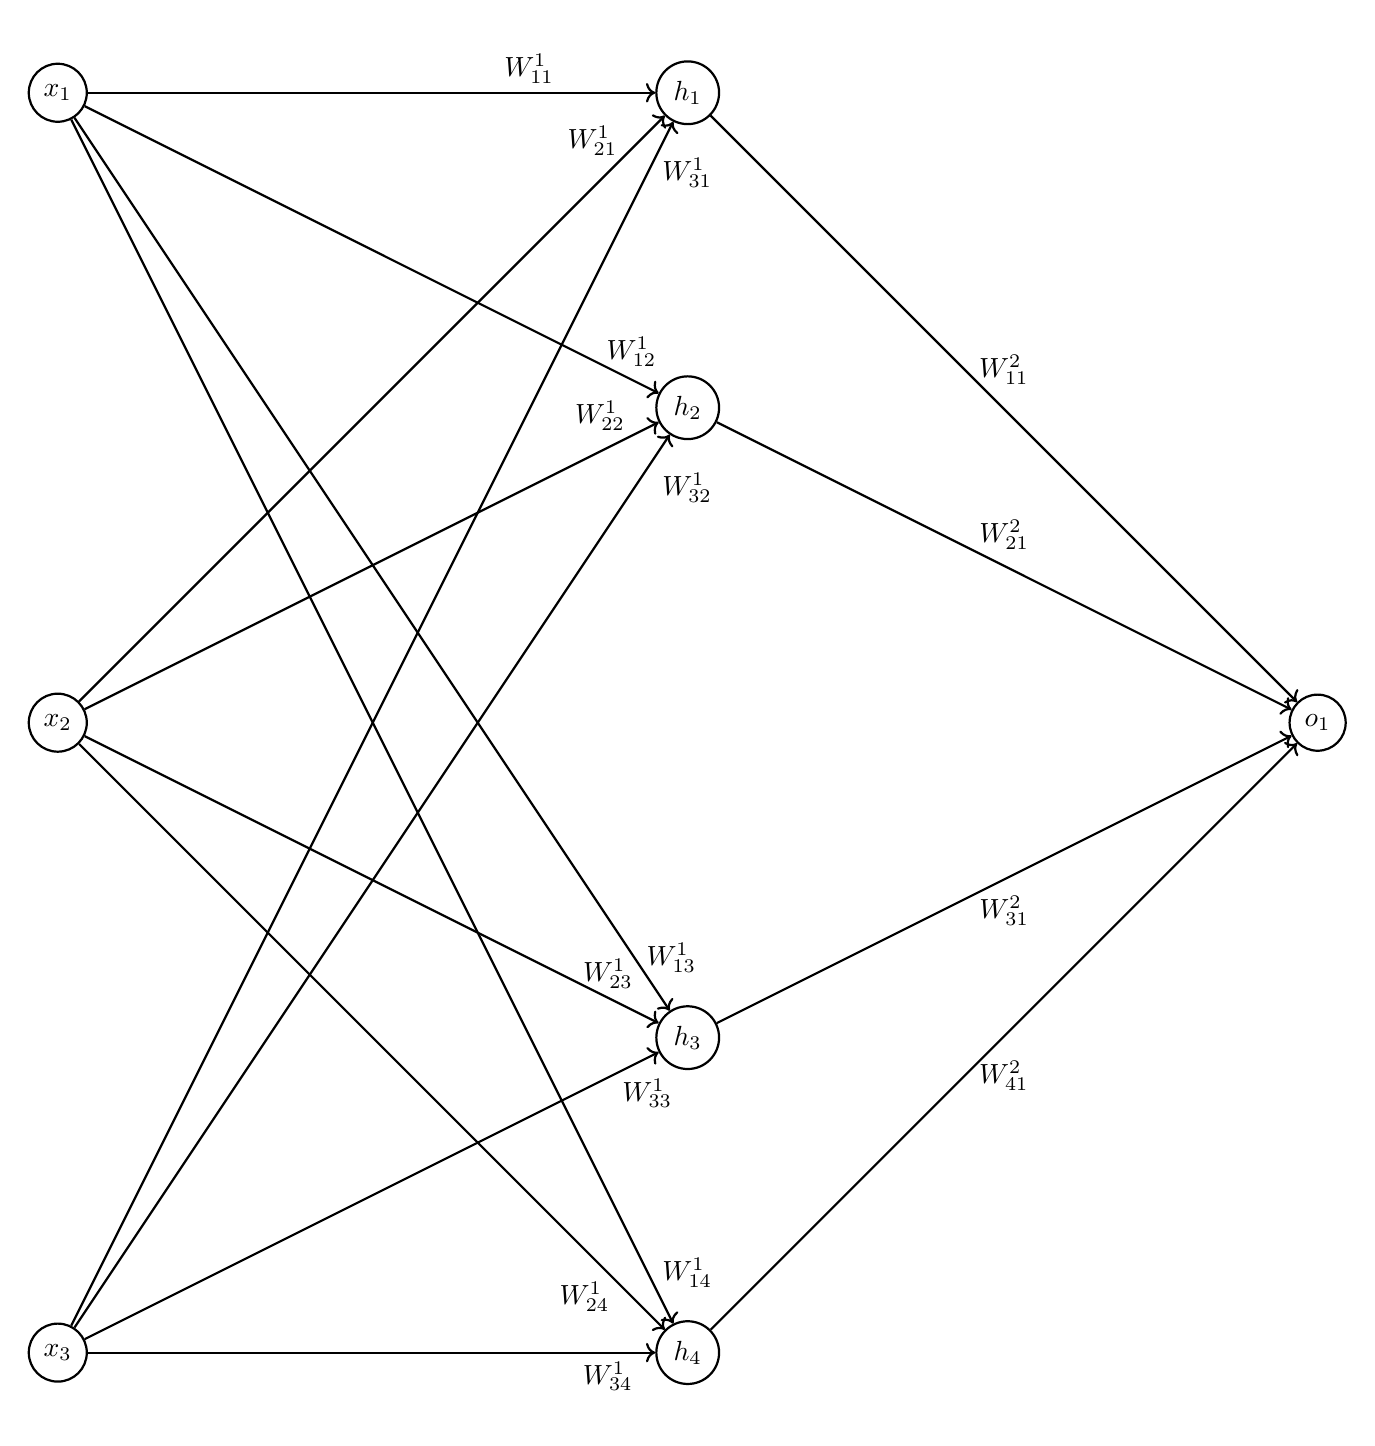
\begin{tikzpicture}
\begin{scope}[every node/.style={circle,thick,draw}]
   \node (x1) at (0,8) {$x_1$};
   \node (x2) at (0,0) {$x_2$};
   \node (x3) at (0,-8) {$x_3$};

   \node (h1) at (8, 8) {$h_1$};
   \node (h2) at (8, 4) {$h_2$};
   \node (h3) at (8, -4) {$h_3$};
   \node (h4) at (8, -8) {$h_4$};

   \node (o1) at (16, 0) {$o_1$};
   %\node (o2) at (8, -1) {$o_2$};
\end{scope}

\begin{scope}[every edge/.style={draw,thick, circle},
             every node/.style={circle}]

   \path [->] (x1) edge node[yshift=0.3cm, xshift=2cm] {$W_{11}^1$} (h1);
   \path [->] (x1) edge node[yshift=-1.3cm, xshift=3.3cm] {$W_{12}^1$} (h2);
   \path [->] (x1) edge node[yshift=-5cm, xshift=3.8cm] {$W_{13}^1$} (h3);
   \path [->] (x1) edge node[yshift=-7cm, xshift=4cm] {$W_{14}^1$} (h4);

   \path [->] (x2) edge node[yshift=3.4cm, xshift=2.8cm] {$W_{21}^1$} (h1);
   \path [->] (x2) edge node[yshift=1.9cm, xshift=2.9cm] {$W_{22}^1$} (h2);
   \path [->] (x2) edge node[yshift=-1.2cm, xshift=3cm] {$W_{23}^1$} (h3);
   \path [->] (x2) edge node[yshift=-3.3cm, xshift=2.7cm] {$W_{24}^1$} (h4);

   \path [->] (x3) edge node[yshift=7cm, xshift=4cm] {$W_{31}^1$} (h1);
   \path [->] (x3) edge node[yshift=5cm, xshift=4cm] {$W_{32}^1$} (h2);
   \path [->] (x3) edge node[yshift=1.3cm, xshift=3.5cm] {$W_{33}^1$} (h3);
   \path [->] (x3) edge node[yshift=-0.3cm, xshift=3cm] {$W_{34}^1$} (h4);

   \path [->] (h1) edge node[yshift=0.5cm] {$W_{11}^2$} (o1);
   \path [->] (h2) edge node[yshift=0.4cm] {$W_{21}^2$} (o1);
   \path [->] (h3) edge node[yshift=-0.4cm] {$W_{31}^2$} (o1);
   \path [->] (h4) edge node[yshift=-0.5cm] {$W_{41}^2$} (o1);

   %\path [->] (h1) edge node {${W^2}_{12}$} (o2);
   %\path [->] (h2) edge node {${W^2}_{22}$} (o2);
   %\path [->] (h3) edge node {${W^2}_{32}$} (o2);
   %\path [->] (h4) edge node {${W^2}_{42}$} (o2);
\end{scope}
\end{tikzpicture}
\caption{A fully connected single-layer artificial neural network.}
\label{fig:ann1}
\end{figure}
\newpage
\subsection{The Forward Pass - A motivating example}
The \textit{Forward Pass}, also sometimes called forward-propagation is the
function that takes in a sample input to the network, and produces
a prediction of the output. The goal of an artificial neural network is to 
minimise the difference between this prediction and the actual output, 
and to ensure that this function can generalise well for new inputs. The
forward pass is shown in figure \ref{fig:ann2} using arbitrary example inputs
and weights, described in the following subsections:
\subsubsection{Example Input}
The input for the example in figure \ref{fig:ann2} is:
$\boldsymbol{x} = \langle 1, 2, 3 \rangle$
\begin{minted}{haskell}
x :: [Double]
x = [1.0, 2.0, 3.0]
\end{minted}
\subsubsection{Example Weights}
The two weight matrices in figure \ref{fig:ann2} are: \\
$\boldsymbol{W}^1 = 
  \begin{bmatrix}
       0.1 && 0.5 && 0.9  \\
       0.2 && 0.6 && 0.25 \\
       0.3 && 0.7 && 0.55 \\
       0.4 && 0.8 && 0.75 \\
  \end{bmatrix} \\
\boldsymbol{W}^2 =
  \begin{bmatrix}
  0.15 && 0.35 && 0.65 && 0.85
  \end{bmatrix}$
\begin{minted}{haskell}
w1 :: [[Double]]
w1 = [[0.1, 0.5, 0.9],
      [0.2, 0.6, 0.25],
      [0.3, 0.7, 0.55],
      [0.4, 0.8, 0.75]]
w2 :: [[Double]]
w2 = [[0.15, 0.35, 0.65, 0.85]]
\end{minted}
\subsubsection{Example Input Function}
The input function used to achieve the results in figure \ref{fig:ann2} is
the matrix-vector multiplication. \\
$\boldsymbol{W}^1 \boldsymbol{x}^T = 
\begin{bmatrix}
   0.1 && 0.5 && 0.9  \\
   0.2 && 0.6 && 0.25 \\
   0.3 && 0.7 && 0.55 \\
   0.4 && 0.8 && 0.75 \\
\end{bmatrix} 
\begin{bmatrix}
   1.0 \\
   2.0 \\
   3.0 
\end{bmatrix}
= \begin{bmatrix}
   3.8 \\
   2.15 \\
   3.35 \\
   4.25
  \end{bmatrix}$
\begin{minted}{haskell}
matVecMultiply :: [[Double]] -> [Double] -> [Double]
matVecMultiply xss ys = fmap (\xs -> sum $ zipWith (*) xs ys) xss

matMatMultiply :: [[Double]] -> [[Double]] -> [[Double]]
matMatMultiplay xss yss = fmap (\xs -> 
   fmap (\ys -> sum $ zipWith (*) xs ys) yss)
\end{minted}
\pagebreak
\subsubsection{Example Activation Function}
Figure \ref{fig:ann2} uses the sigmoid activation function. \\
$S(x) = \frac{1}{1 + e^{-x}} \\
 S_v(\boldsymbol{x}) = [S(x_i)], \forall x_i \in \boldsymbol{x}$
\begin{minted}{haskell}
sigmoid :: [Double] -> [Double]
sigmoid xs = 
   let s = 1 / (1 + exp (negate x))
   in fmap s xs
\end{minted}
\subsubsection{Example Hidden Layer}
The hidden layer in figure \ref{fig:ann2} applies the input function and the
activation to the inputs and weights. \\
$ \boldsymbol{z} = \boldsymbol{W}^1 \boldsymbol{x}^T = 
\begin{bmatrix}
   3.8 \\
   2.15 \\
   3.35 \\
   4.25
  \end{bmatrix} \\
\boldsymbol{a}^1 = S_v(\boldsymbol{z}) \approx \begin{bmatrix}
   0.97812 \\
   0.89567 \\
   0.96611 \\
   0.98594
   \end{bmatrix}$
\begin{minted}{haskell}
a1 :: [Double] -> [Double]
a1 = sigmoid

h1 :: [[Double]] -> [Double] -> [Double]
h1 wss xs = a1 $ matVecMultiply wss xs
\end{minted}

\subsubsection{Example Output Layer}
The output layer uses the same matrix-vector multiplication (or specifically in
the case of figure \ref{fig:ann2}, a vector-vector multiplication). However the
output layer for a regression problem does not normally have a sigmoid
activation, and instead simple has the id function as it's activation. \\
$\boldsymbol{z}^2 = \boldsymbol{W}^2 \boldsymbol{a}^1 = 
\begin{bmatrix}
   0.15 && 0.35 && 0.65 && 0.85
\end{bmatrix}
\begin{bmatrix}
 0.97812 \\
   0.89567 \\
   0.96611 \\
   0.98594
\end{bmatrix} \approx 1.92623 \\
\boldsymbol{a}^2(\boldsymbol{x}) = \boldsymbol{x} \\
\boldsymbol{a}^2(\boldsymbol{z}^2) = \boldsymbol{z}^2$

\begin{minted}{haskell}
vecVecMultiply :: [Double] -> [Double] -> [Double]
vecVecMultiply xs ys = sum $ zipWith (*) xs ys

a2 :: [Double] -> [Double]
a2 = id

o1 :: [Double] -> [Double] -> [Double]
o1 ws as = a2 $ vecVecMultiplay ws as
\end{minted}

\newpage
\begin{figure}[h]
   \centering
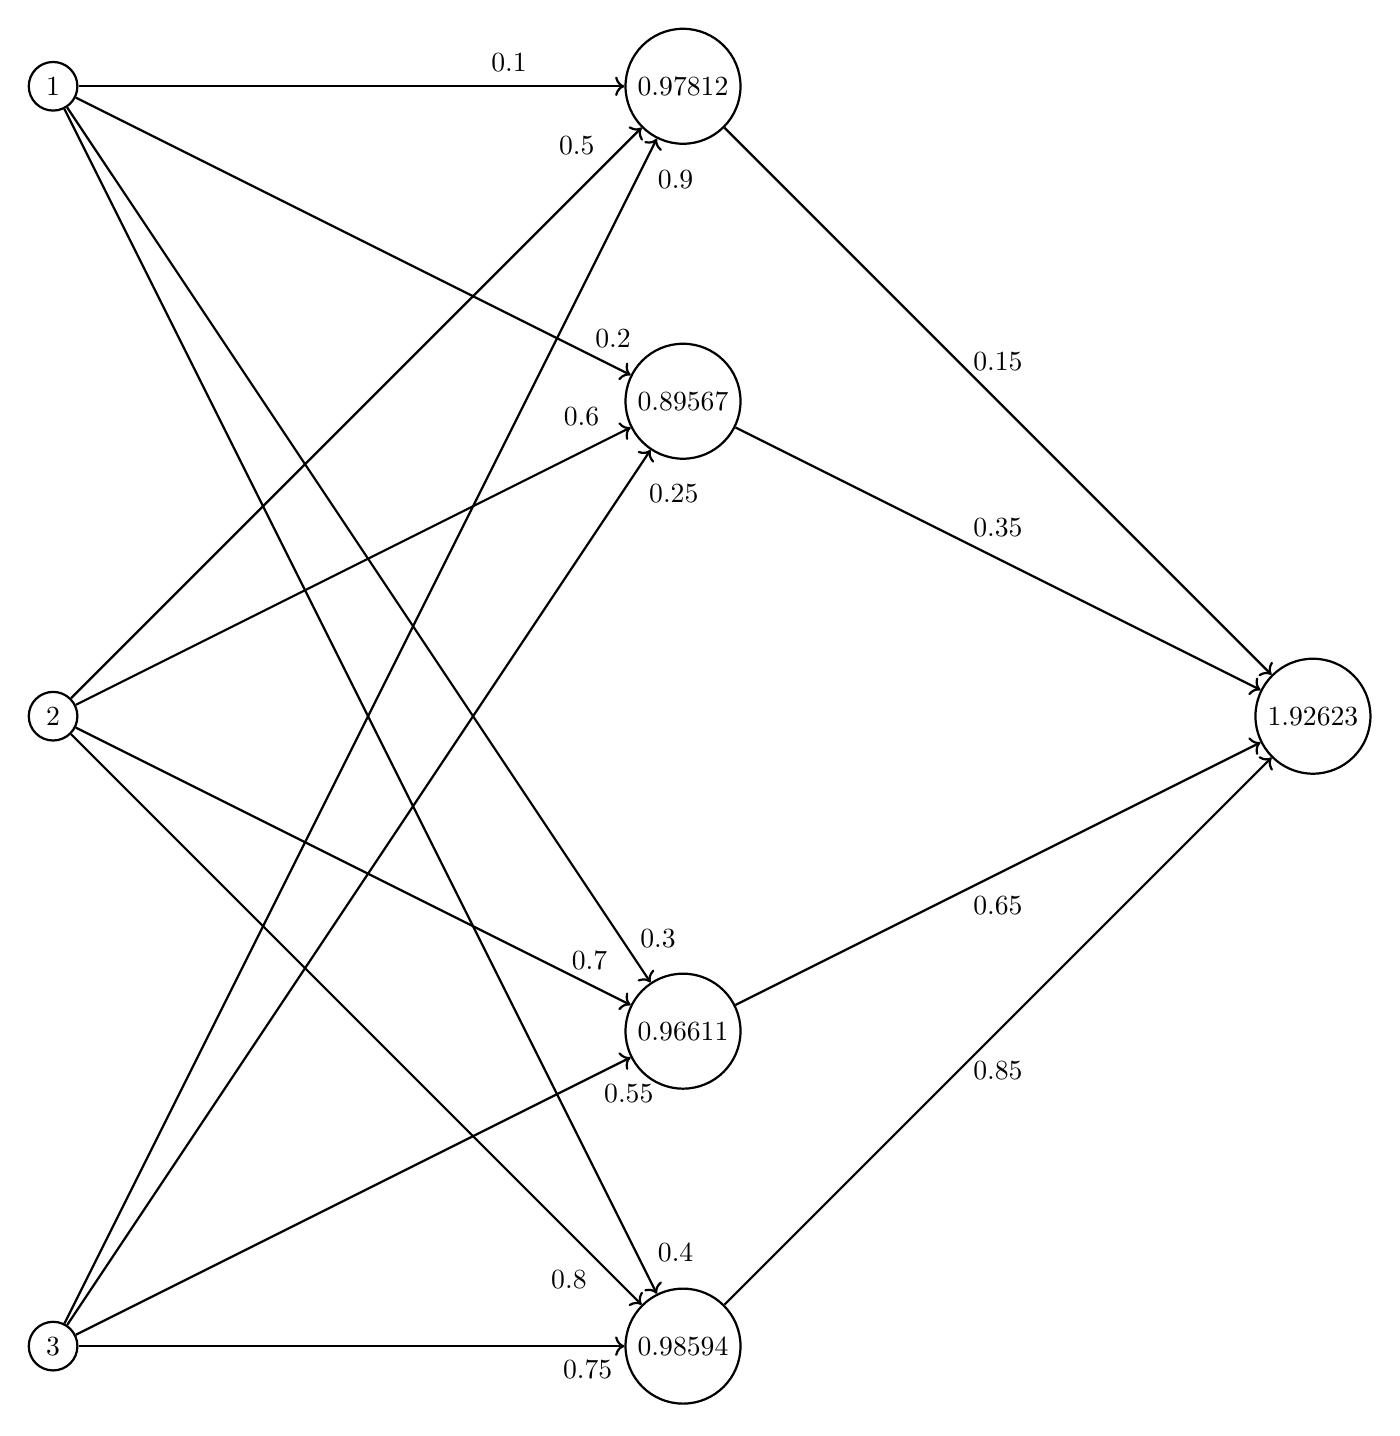
\begin{tikzpicture}
\begin{scope}[every node/.style={circle,thick,draw}]
   \node (x1) at (0,8) {$1$};
   \node (x2) at (0,0) {$2$};
   \node (x3) at (0,-8) {$3$};

   \node (h1) at (8, 8) {$0.97812$};
   \node (h2) at (8, 4) {$0.89567$};
   \node (h3) at (8, -4) {$0.96611$};
   \node (h4) at (8, -8) {$0.98594$};

   \node (o1) at (16, 0) {$1.92623$};
   %\node (o2) at (8, -1) {$o_2$};
\end{scope}

\begin{scope}[every edge/.style={draw,thick, circle},
             every node/.style={circle}]

   \path [->] (x1) edge node[yshift=0.3cm, xshift=2cm] {$0.1$} (h1);
   \path [->] (x1) edge node[yshift=-1.3cm, xshift=3.3cm] {$0.2$} (h2);
   \path [->] (x1) edge node[yshift=-5cm, xshift=3.8cm] {$0.3$} (h3);
   \path [->] (x1) edge node[yshift=-7cm, xshift=4cm] {$0.4$} (h4);

   \path [->] (x2) edge node[yshift=3.4cm, xshift=2.8cm] {$0.5$} (h1);
   \path [->] (x2) edge node[yshift=1.9cm, xshift=2.9cm] {$0.6$} (h2);
   \path [->] (x2) edge node[yshift=-1.2cm, xshift=3cm] {$0.7$} (h3);
   \path [->] (x2) edge node[yshift=-3.3cm, xshift=2.7cm] {$0.8$} (h4);

   \path [->] (x3) edge node[yshift=7cm, xshift=4cm] {$0.9$} (h1);
   \path [->] (x3) edge node[yshift=5cm, xshift=4cm] {$0.25$} (h2);
   \path [->] (x3) edge node[yshift=1.3cm, xshift=3.5cm] {$0.55$} (h3);
   \path [->] (x3) edge node[yshift=-0.3cm, xshift=3cm] {$0.75$} (h4);

   \path [->] (h1) edge node[yshift=0.5cm] {$0.15$} (o1);
   \path [->] (h2) edge node[yshift=0.4cm] {$0.35$} (o1);
   \path [->] (h3) edge node[yshift=-0.4cm] {$0.65$} (o1);
   \path [->] (h4) edge node[yshift=-0.5cm] {$0.85$} (o1);

   %\path [->] (h1) edge node {${W^2}_{12}$} (o2);
   %\path [->] (h2) edge node {${W^2}_{22}$} (o2);
   %\path [->] (h3) edge node {${W^2}_{32}$} (o2);
   %\path [->] (h4) edge node {${W^2}_{42}$} (o2);
\end{scope}
\end{tikzpicture}
\caption{A neural network using linear-combination, sigmoid and id.}
\label{fig:ann2}
\end{figure}
\newpage

\subsection{Artificial Neural Networks - The Training Step} \label{training}
\textit{Training}, \textit{Learning}, \textit{Back-prop} -- these are all 
common colloquial expressions used to describe the process of optimising 
the weights of the network with regard to the error of the network. 
That is, which values of weights in the
network will result in the most accurate, and most general, results in the
forward pass. Despite the names given here, any optimisation method that
can minimise the error with regard to the weights can be used for this task.
Including: genetic algorithms, newton's multivariate root finding method, 
particle swarm optimisation, and so on. 
\text{Back-prop} comes from the arguably 
most-common optimisation methods, gradient descent and stochastic gradient
descent.

\subsubsection{Stochastic Gradient Descent and Back Propagation}
Stochastic gradient descent is an algorithm that attempt to minimise the error
of the network by calculating the gradient of the weights with respect to this
error, in a step often known as \textit{Back Propagation}. This 'propagates'
the error from the forward pass back through the network using the chain rule
to find the gradient of the weights. The gradients for the
network shown in figures \ref{fig:ann1} and \ref{fig:ann2} are:

\begin{align*}
				\frac {\partial c^r}{\partial \boldsymbol{W}^2} &= 
						\frac{\partial c^r}{\partial o^r} \frac{\partial o^r}{\partial
						\boldsymbol{z}^2} \frac{\partial \boldsymbol{z}^2}{\partial
						\boldsymbol{W}^2} \\
				\frac{\partial c^2}{\partial \boldsymbol{W}^1} &= 
						\frac{\partial c^r}{\partial o^r} \frac{\partial o^r}{\partial
						\boldsymbol{z}^2} \frac{\partial \boldsymbol{z}^2}{\partial
						\boldsymbol{a}^1} \frac{\partial \boldsymbol{a}^1}{\partial
						\boldsymbol{z}^1} \frac{\partial \boldsymbol{z}^1}{\partial
						\boldsymbol{W}^1}
\end{align*}

Once the gradients of the weights with respect to the error of the network 
have been calculated, the previous weights are updated by subtracting the
partial in each element of the gradient matrix, from the element in the
original matrix, multiplied by a learning rate $\alpha$:

\begin{align*}
				f(\boldsymbol{X}^{mn}, \boldsymbol{Y}^{mn}) = x_{ij} - \alpha y_{ij}, 
				\forall x \in \boldsymbol{X}, \forall y \in \boldsymbol{Y}
\end{align*}

Finally, in stochastic gradient descent this process is repeated for each 
training example, and then started again, until a specified number of
iterations have passed. By contrast, ordinary gradient descent operates
on all the training examples at once, and takes the gradient of the whole
network (as a matrix or tensor), and updates the weights in one large step.
This is usually less common in practice due to memory constraints.

\section{Specification} \label{specification}
The implementation consists of two executable programs. A learning subsystem 
BANNHL (A Back-propagating Artificial Neural Network in Haskell: Learner) 
which learns the weights from supplied training data and network structure, 
and a 
classification/prediction subsystem BANNHC (A Back-propagating Artificial Neural Network in Haskell:
Classifier) which classifies a given example according to a learned 
model. The specifics of the inputs and outputs to these programs now follows.

\subsection{Learning a model from training data.}
The training application (BANNH) requires several inputs from the 
user: 
\begin{itemize}
   \item Training Data Path: The path to the file containing the training 
      data, in csv format. 
   \item Weights File Path: The path to the file where the user would like 
      the learned weights saved to.
   \item Number of Epochs: The number of epochs (iterations) to run the
      stochastic gradient descent algorithm. This must be an Integer value.
   \item The Learning Rate: The learning rate (alpha) the user would
      like the stochastic gradient descent algorithm to use. This must be
      a decimal point value.
\end{itemize}

It will then save the weights to the specified location (overwriting any
existing data!), which can be used with BANNHC to classify or predict values
from the problem file. The following depicts running the training application
from a bash terminal on a Linux system. 
\begin{code}
\captionof{listing}{Running the training application from a bash prompt.}
   \begin{minted}[frame=single,framesep=10pt]{bash}
   ./BANNHL training-data.csv weights.txt 1000 0.05
   \end{minted}
\end{code}

\subsubsection{The Training Data File}
The training data must be supplied in the form of a csv file, with no
annotations or comments. Subject to the following conventions:

\begin{itemize}
   \item A single instance of a training example must fit on one line.
   \item By convention the last comma-separate element on this line is
   the label, or correct value for the example.
   \item All training instances must have the same number of comma separated
   values (i.e they must be the same length).
\end{itemize}

Below is an example training data for the function 
$\{x^2 | {-5} \leq x \leq 5\}$. \\
\begin{code}
\captionof{listing}{An example of training data.}
    \begin{minted}[frame=single,framesep=10pt]{haskell}
    -5, 25
    -4, 16
    -3, 9
    -2, 4
    -1, 1
    0, 0
    1, 1
    2, 4
    3, 9
    4, 16
    5, 25
    \end{minted}
\end{code}

\subsubsection{The Weights File}
The weights file is a list of weights for each layer in the network, this
file is automatically generated by the program, and any manual alterations
could cause exceptions at worst, or different classification and prediction
results at best.
The file also contains the maximum value for the training data vector, and the
maximum value for the label vector. This allows normalised data sets to be
unnormalised in the classification application (BANNHC). 
Please also note that the example below has had new lines inserted for display 
purposes. and does not quite reflect the actual format of the weights file.

\begin{code}
\captionof{listing}{An example of the weights file.}
   \begin{minted}[frame=single,framesep=10pt]{haskell}
   ([
     [-1.4964992967401658,-0.26537212688625034,-1.0474151328081605,
      -1.0225725955754879,-3.8958706816175863,-2.452754168685296,
      -0.48799398042475217,-1.2702459797432 561,1.1520590658517951e-2,
      -1.3657344291492945,-1.3868499588233776,-0.34231457119567266,
      -1.3489399072539803,-0.8895707083221474,-0.6831976914228292,
      -0.6785299641374357,-3.1183619929959816,-2.1052816032598325,
      -0.9063554174987992,-0.45763264641324564
     ],
     [-1.1620086785757628,-0.689972750930609,1.9502469317118758,
      -0.10625975742691744,0.23070762147355328,-0.9451163847612435,
      -0.42911096525272274,-0.20284750154931844,1.1424231101169038,
      -0.36909509644044697,1.1176981166123088]
    ],(100.0,10000.0))
   \end{minted}
\end{code}

\subsection{The Classification Application}
The BANNHC executable takes the weights file created by BANNHL as the input,
along with a 'problem' file, that is: a file containing a list of function
inputs for which the classification application will predict the correct value.

\begin{code}
\captionof{listing}{Running the classification application from a bash prompt.}
   \begin{minted}[frame=single,framesep=10pt]{bash}
   ./BANNHC weights.txt problems.txt
   \end{minted}
\end{code}


\subsubsection{The Problem File}
The problem file must be in a text format adhering to the following rules for a
successful read:
\begin{itemize}
   \item The input vector, or scalar of the values you'd like to predict the
      output/classification for, as a single entry on a line.
   \item All lines must contain the same length vector, or solely a scalar.
   \item A separate file must be created for each function, there can be no
      mixing of function inputs (i.e some lines vectors, others as scalars).
\end{itemize}

\pagebreak

\begin{code}
\captionof{listing}{An example of a problem file for $x^2$.}
   \begin{minted}[frame=single,framesep=10pt]{haskell}
   1
   -2
   3
   -5
   \end{minted}
\end{code}

\subsubsection{The output of the classification application}
The output of BANNHC will consist of each line in the problem file, with the
classification according to the learned model, expressed an (input, output) 
tuple.

\begin{code}
\captionof{listing}{An example of output for $x^2$.}
   \begin{minted}[frame=single,framesep=10pt]{haskell}
   (1.0,0.9791312539008473)
   (-2.0,4.008406843304866)
   (3.0,8.76928687144041)
   (-5.0,24.88141526123177)
   \end{minted}
\end{code}

\section{Implementation} \label{implementation}
This section discuss some of the key implementation details in
BANNHL and BANNHC, along with the specific on how to configure the 
structure of the artificial neural network through modifying the 
NNConfig.hs file (the NNConfig module). 
\subsection{NNConfig - Parameters for network structure}
This module has four small functions: sizes, layers, applyFuncs, and cost
(see NNConfig.hs in the Appendix for details). Each of these functions
has a significant impact on the structure of the neural network:

\subsubsection{sizes}
\begin{minted}{haskell} 
sizes :: [Size Int]
\end{minted}
This function is simply a list of integer tuples in Haskell,
however this is subject to some network design rules that specifically
affect the size of the weights matrix, the number of layers (and therefore
the number of weight matrices), and the allocation of bias nodes.
   \begin{enumerate}
     \item The number of tuples is the number of layers in the network if
     the network is solving a classification problem.
     \item The number of tuples is the number of layers in the network minus
     one if the network is solving a regression problem.
     \item The typical bias setup for an artificial neural network places an
     extra neuron for each on the input to the layer (the first value in each
     tuple), this is represented by incrementing the number by one.
   \end{enumerate}
In particular the sizes function is used by the setWeights function in BANNHL
to allocate the size and number of weight matrices for the network.

\subsubsection{layers}
\begin{minted}{haskell} 
layers :: [Layer a]
\end{minted}
Similar to sizes, this is a list of layers (see NNTypes.hs in the appendix,
lines 14-15). The goal of this function is to provide a list of different layer
types (excluding the 'cost' layer) that depict the compositional operations
throughout the network. Currently only the 'fully connected' layer is defined
in NNLayers (Appendix - NNLayers.h, lines 17-18), which is the most common type
of layer structure, however it leaves scope for more advanced types of layers
(convolution, etc) to be added in the future. Note that any new layers created
\textit{must} be exported from NNLayers.hs and imported in NNConfig.hs!
\begin{enumerate}
   \item If the network requires a substantially different final layer, reduce
   the value of the argument to replicate by one.
\end{enumerate}

\subsubsection{applyFuncs}
\begin{minted}{haskell}
applyFuncs :: (Floating a) => [Vector a -> Vector a -> Vector a]
\end{minted}
applyFuncs is another network structure building function, it uses the
prepLayer function from NNLayers to restructure the network into a list of
weights to inputs to outputs, this is key to BANNHL's approach of currying
the forward pass results through the network, and then taking the derivative
with regard to the weights. 
\begin{enumerate}
   \item To change the network from classification to regression (particularly
   if using a Sigmoid activation function), append the prepLayer function using
   an id instead of the normal activation function. This also must coincide
   with reducing the length of layers by 1.
   \item To change the network from regression to classification, delete or
   uncomment the \textbf{++ prepLayer sp id layers} on line 37 of NNLayers.hs. 
\end{enumerate}

\subsubsection{cost}
\begin{minted}{haskell}
cost :: (Floating a, Ord a) => Vector a -> [Vector a-> Vector a]
\end{minted}
cost takes in the labels, or actuals for the training example, it then curries
the the actuals, and the specified cost function through the costLayer
generation function. To change the error function in the costLayer simply
replace sError with one of the other cost functions that have been imported
from NNCostFuncs.

\subsection{NNForwardPass - The output of the network}
The NNForwardPass module implements a slightly different forward pass than
what is traditionally seen from the mathematical descriptions of the algorithm,
notably it does not implement the cost function or get the error value, the
forward pass simply calculates the output of the network via the following
functions.

\subsubsection{applyWeights}
\begin{minted}{haskell}
applyWeights :: (Floating a) => [Vector a] -> [Vector a -> Vector a]
\end{minted}
applyWeights applies each element of it's argument to the function
applyFuncs from NNConfig, this returns a list of layer inputs to
layer outputs, which can than be easily scanned to display the forward pass.

\subsubsection{fp}
\begin{minted}{haskell}
fp :: (Floating a) => Vector a -> [Vector a] -> [Vector a]
\end{minted}
fp, short for forward pass, takes the inputs to the network, and a list
of weights for the network, using the function applyWeights above, produces
a list of each layers output values, this is important to use for the backwards
pass in BANNHL.

\subsection{BANNHL - The back-propagating neural network}
BANNHL is responsible for thee broad tasks: calculate derivatives of functions,
initialise random weights for the network, and to perform stochastic gradient
descent. Rather than calculate the Jacobian matrix for each layer manually,
and force the user to update every function with it's derivative should they
decide to change activation functions, for instance, an automatic
differentiation approach was chosen, using Haskell's \textbf{ad} library 
~\cite{Elliott2009-beautiful-differentiation}.

\subsubsection{deriveWeights}
\begin{minted}{haskell}
deriveWeights :: (Floating a, Ord a) => 
   [ [AD.Khan a] -> [AD.Khan a] ] -> [ [a] -> [[a]] ]
\end{minted}
deriveWeights is responsible for evaluating the derivative of all the weights
in the network with respect to the error of the network, it does this by
simply mapping AD.jacobian over a list of functions
\mintinline{haskell}{[SomeWeights -> SomeError]}. 
Despite being a deceptively terse function, BANNHL spends most of the CPU
time inside deriveWeights via the Kahn mode automatic differentiation.

\subsubsection{backProp}
\begin{minted}{haskell}
backProp :: (Floating a, Ord a) =>
   Vector a ->
   [Vector a] ->
   [Vector a] ->
   [Vector a -> Vector a -> Vector a] ->
   [Vector a -> Vector a]
\end{minted}
backProp takes the actuals, weights, inputs and network (where the network is
in the form of \\
\mintinline{haskell}{[LayerInputs -> LayerWeights ->
LayerOutput]}) and produces a list of functions from weights to error.
It does this by flipping the arguments of the current item in the function
vector and then folding composition through the reverse function vector.
This generate a function weights to error, backProp then operates recursively
on the tails of all the input lists (see lines 59-64 BANNHL.hs in the
appendix).

\section{Demonstration}
This section details a working example of the neural network.
\subsection{The training data}
The training data for $x^2$ this may not generalise well for functions outside
of the data here, but is sufficient to prove network convergence.
\begin{code}
\captionof{listing}{smallXSquared.csv}
   \begin{minted}[frame=single,framesep=10pt,linenos]{bash}
   -5, 25
   -4, 16
   -3, 9
   -2, 4
   -1, 1
   0, 0
   1, 1
   2, 4
   3, 9
   4, 16
   5, 25
   \end{minted}
\end{code}

\subsection{Executing the training application on smallXSquared.csv}
Note, the weights are random, so it may take several restarts to get
a satisfactory prediction - If the first entry in the list is 1.0, then
the last should be as close to 1.0 as possible.
\begin{code}
\captionof{listing}{running the training application.}
   \begin{minted}[frame=single,framesep=10pt,linenos]{bash}
   ./BANNHL smallXSquared.csv results.txt 5000 0.22
   [[1.0],[0.31324279308679365,2.8615624029093333e-3,0.3319068121863323,
    0.4058300654339911,0.6171955038138789,0.36871023930970587,
    0.5316629601588719,0.4456624330308043,0.44508288056808964,
    0.16923045656208946],[0.9996381532479468]]
   \end{minted}
\end{code}

\subsection{The problem file for the classification application}
A small number of problems for the $x^2$ network.
\begin{code}
\captionof{listing}{problems.txt}
   \begin{minted}[frame=single,framesep=10pt,linenos]{bash}
   1
   -2
   3
   -5
   2.5
   \end{minted}
\end{code}

\subsection{Executing the classification application}
Running BANNHC with the results.txt from BANNHL, and problems.txt.
\begin{code}
\captionof{listing}{Running BANNHC.}
   \begin{minted}[frame=single,framesep=10pt,linenos]{bash}
   ./BANNHC results.txt problems.txt 
   (1.0,0.9791223417057613)
   (-2.0,3.97472811919036)
   (3.0,8.94344963037105)
   (-5.0,24.98932320484025)
   (2.5,6.131835625576089)
   \end{minted}
\end{code}

\section{Challenges and Future Work} \label{challenges}
This section discusses challenges encountered during this implementation 
process along with any identifiable areas for future work.

\subsection{Improvements to BANNH}
While this report has demonstrated that BANNH can learn and predict simple
mathematical functions to a given degree of accuracy, neural network models
have a large number of parameters (learning rate, network structure, number of
epochs, and network composition) which can vary the results. Further
investigation could be done to empirically support specific network
configurations for specific problem types. To improve BANNH, some work can be 
done in the configurations (NNConfig.hs) file
to lift out the functions used in the function body, to an argument of the
function calling, for example, the cost function could be expressed as an
argument to cost (NNConfig.hs, line 44) instead of manually placed inside the
function, however it has been left this way due to time constraints.
Additional testing can also be done with more complex function types,
validating the implementation for classification problems, and for larger 
problem types.

\subsection{Challenges with Haskell}
As part of an exercise to push the working BANNH implementation to classify
images, an NNImageIO module was implemented, allowing the network to read in
lists of raw pixel values (grey-scale) and attempt to classify the image as an
"X" or an "O". Unfortunately, the implementation suffered a \textit{severe}
degradation in performance when this was tried, taking over ten hours to
complete a single epoch with 60 images. Profiling and heap analysis revealed
this to be almost entirely garbage collection time, the profile suggests that
these allocations are coming primarily from the use of the `ad` library in
haskell, and `ad`'s internal use of the `reflection` library. These libraries
result in a large number of allocations, making the program significantly less
efficient. To support this, a manual neural network prototype was constructed
where all the derivatives were calculated by hand, and a single backwards pass
was run over all 60 images. This implementation only took 60 seconds to run a
single epoch, unfortunately manually differentiating the network requires a lot
of time and maintenance and does not scale well for larger networks.

There is a lot that could be improve with regard to the Haskell implementation
of BANNH:
\begin{itemize}
   \item Replacing lists with more efficient data structures (such as those in
   the `vector` library) could help reduce the number of allocations
   ~\cite{gill2000debugging}.
   \item Replacing the `ad` library with an improved differentiation library
   that does not require so many allocations ~\cite{zimmer2006functional}.
   \item The use of 'streams' may result in faster compiler optimisation of the
   recursive functions in BANNHL particularly `learn` and `sgd`
   ~\cite{ida1983functional}.
   \item Using unboxed primitives, and re-writing the implementation to avoid
   re-boxing them could result in fewer allocations
   ~\cite{chakravarty2003approach}.
   \item Incremental Computation could be examined to assist in the memoization
   of functions with similar arguments
   ~\cite{Elliott-2017-compiling-to-categories}.
   \item Finally, naively implementing optimisation algorithms designed in, and
   for, languages that rely on mutable state may not be the best way to 
   implement those algorithms in a purely functional, lazy evaluation 
   environment. Further work may be done to examine if there are more 
   appropriate functionally pure alternatives to the existing algorithms.
\end{itemize}

\section{Conclusion}
BANNH is a successful implementation of an artificial neural network in
Haskell, that uses the back-propagation algorithm to optimise the weights with
respect to the network error. The network successfully achieves convergence,
that is the predictions get progressively more accurate for a given function
provided there is enough sample data, and correct network structure and
parameters are chosen (This has been demonstrated with the function $x^2$ in
section \ref{specification}). BANNH made use of an automatic differentiation
library which provided good asymptotic performance based on the side of the
input, unfortunately the run-time performance of lazy data structures was not
taken into account by the designer of this library, and by the author of BANNH,
resulting in extremely poor scalability when trained for larger classification
problems. Never-the-less BANNH successfully demonstrates that the author has
achieved a level of competency in the Haskell programming language, and in the
functional programming paradigm. 

Going forward, a re-design of BANNH is necessary to achieve acceptable
performance on real-world problems, and an examination of the various
differentiation methods (symbolic, manual, automatic) are required to determine
the most acceptable trade-off between usability and training-time performance.


\section{Author's Reflections} \label{reflection}
I have found this advanced topic in Functional Programming to be both extremely
challenging, and richly rewarding. I would liken the learning-curve to the
experience I had with learning to code for the first time, ever. I suspect this
is because functional programming requires unlearning all the ideas that I
was taught in an undergraduate career of imperative and object-oriented
programming.

I spent the first month of the Trimester fighting with the compiler, and slowly
trying to understand how things work in a functionally pure environment. The
second month was spent trying to understand the RankNTypes extension, in order
to unify my type with the \textbf{ad} library, I never did solve this 
problem, it
turned out that the \textbf{ad} library offered more primitive methods that 
didn't require the RankNTypes extension, but attempting to fix this taught 
me a lot about impredicative types, reification, reflection, data, newtypes,
and type classes as I struggled to resolve the issue. 

The third month was spent actually developing the
details of the artificial neural network. In particular I'd like to note that
programming in a functionally pure environment forced me to think about
artificial neural networks quite differently! Previously when I had read about
their compositional and structure, I mentally started breaking the problem down
into objects, and inheritance relations. This is a poor abstraction, by
visualising the network as a function, and exploiting currying, I was able to
restructure a network to get the gradient of the weights with respect to the
error with minimal effort! This was an eye-opening experience for me.

Finally, as I produced this document, I had to re-factor the majority of my 
code
to fit in with my prescribed specification, in an object-oriented language,
this would've been a nightmare, as classes often inherit or share mutable
state. However in a purely functional paradigm, it was simple a matter of
shifting functions around and ensuring each module had the correct imports and
exports, the entire exercise maybe took ten minutes!

While I feel I have reached an intermediate level in Haskell during the time
spent on this course, I also feel like I have barely scraped the surface of
useful functional abstractions! Even now I am slowly realising that there are 
shorter and more concise methods of writing code that is isomorphic to
to some of my more verbose code. When I started I would
reach for map, resulting in the common pattern:
\begin{minted}{haskell}
fxs = zip fs xs
xs = map ((f, x) -> f x) fxs
\end{minted}
Which is really instead just:
\begin{minted}{haskell}
xs = zipWith ($) fs xs
\end{minted}
This is just one example of the many isomorphisms I've discovered, either as my
own knowledge has grown, or through the use of hint tools such as hlint.

Finally, I would like to touch on how easy it was to prototype in Haskell,
it took only an hour to build a working artificial neural network where I
performed the back-propagation calculations from scratch! I had spent more time
checking and double checking my mathematics than actually implementing the
code!

All in all, this course has opened my eyes to the power and flexibility of
functional programming, and also presented me with a strong focus for future
research in the area of performance optimisation for common algorithms in
artificial intelligence.
\bibliography{references.bib}{}
\bibliographystyle{apalike}

\appendix
\section{Appendix A - Source Code}
\subsection{BANNHC and BANNHL}
\begin{code}
\captionof{listing}{NNTypes - Types.}
   \inputminted[frame=single,framesep=10pt,linenos]{haskell}
   {../src/NNTypes.hs}
\end{code}

\begin{code}
\captionof{listing}{NNUtils - Utility functions.}
   \inputminted[frame=single,framesep=10pt,linenos]{haskell}
   {../src/NNUtils.hs}
\end{code}

\begin{code}
\captionof{listing}{NNFileIO - Reading data from files.}
   \inputminted[frame=single,framesep=10pt,linenos]{haskell}
   {../src/NNFileIO.hs}
\end{code}

\begin{code}
\captionof{listing}{NNConfig - Manual Configuration of the network.}
   \inputminted[frame=single,framesep=10pt,linenos]{haskell}
   {../src/NNConfig.hs}
\end{code}

\begin{code}
\captionof{listing}{NNLayers - Layer configurations available to the network.}
   \inputminted[frame=single,framesep=10pt,linenos]{haskell}
   {../src/NNLayers.hs}
\end{code}

\begin{code}
\captionof{listing}{NNCostFuncs - Cost Functions available to the network}
   \inputminted[frame=single,framesep=10pt,linenos]{haskell}
   {../src/NNCostFuncs.hs}
\end{code}

\begin{code}
\captionof{listing}{NNInputFuncs - Input Functions available to the network}
   \inputminted[frame=single,framesep=10pt,linenos]{haskell}
   {../src/NNInputFuncs.hs}
\end{code}

\begin{code}
\captionof{listing}{NNActivationFuncs - Activation Functions available to the 
   network}
   \inputminted[frame=single,framesep=10pt,linenos]{haskell}
   {../src/NNActivationFuncs.hs}
\end{code}

\begin{code}
\captionof{listing}{NNForwardPass - The forward pass through the network.}
   \inputminted[frame=single,framesep=10pt,linenos]{haskell}
   {../src/NNForwardPass.hs}
\end{code}

\begin{code}
\captionof{listing}{BANNHL - Backpropgation 'learner'.}
   \inputminted[frame=single,framesep=10pt,linenos]{haskell}
   {../src/BANNHL.hs}
\end{code}

\begin{code}
\captionof{listing}{BANNHC - 'classifier'}
   \inputminted[frame=single,framesep=10pt,linenos]{haskell}
   {../src/BANNHC.hs}
\end{code}

\newpage
\section{Appendix B - Performance of BANNHL}
\subsection{Heap Profiles for BANNHL}
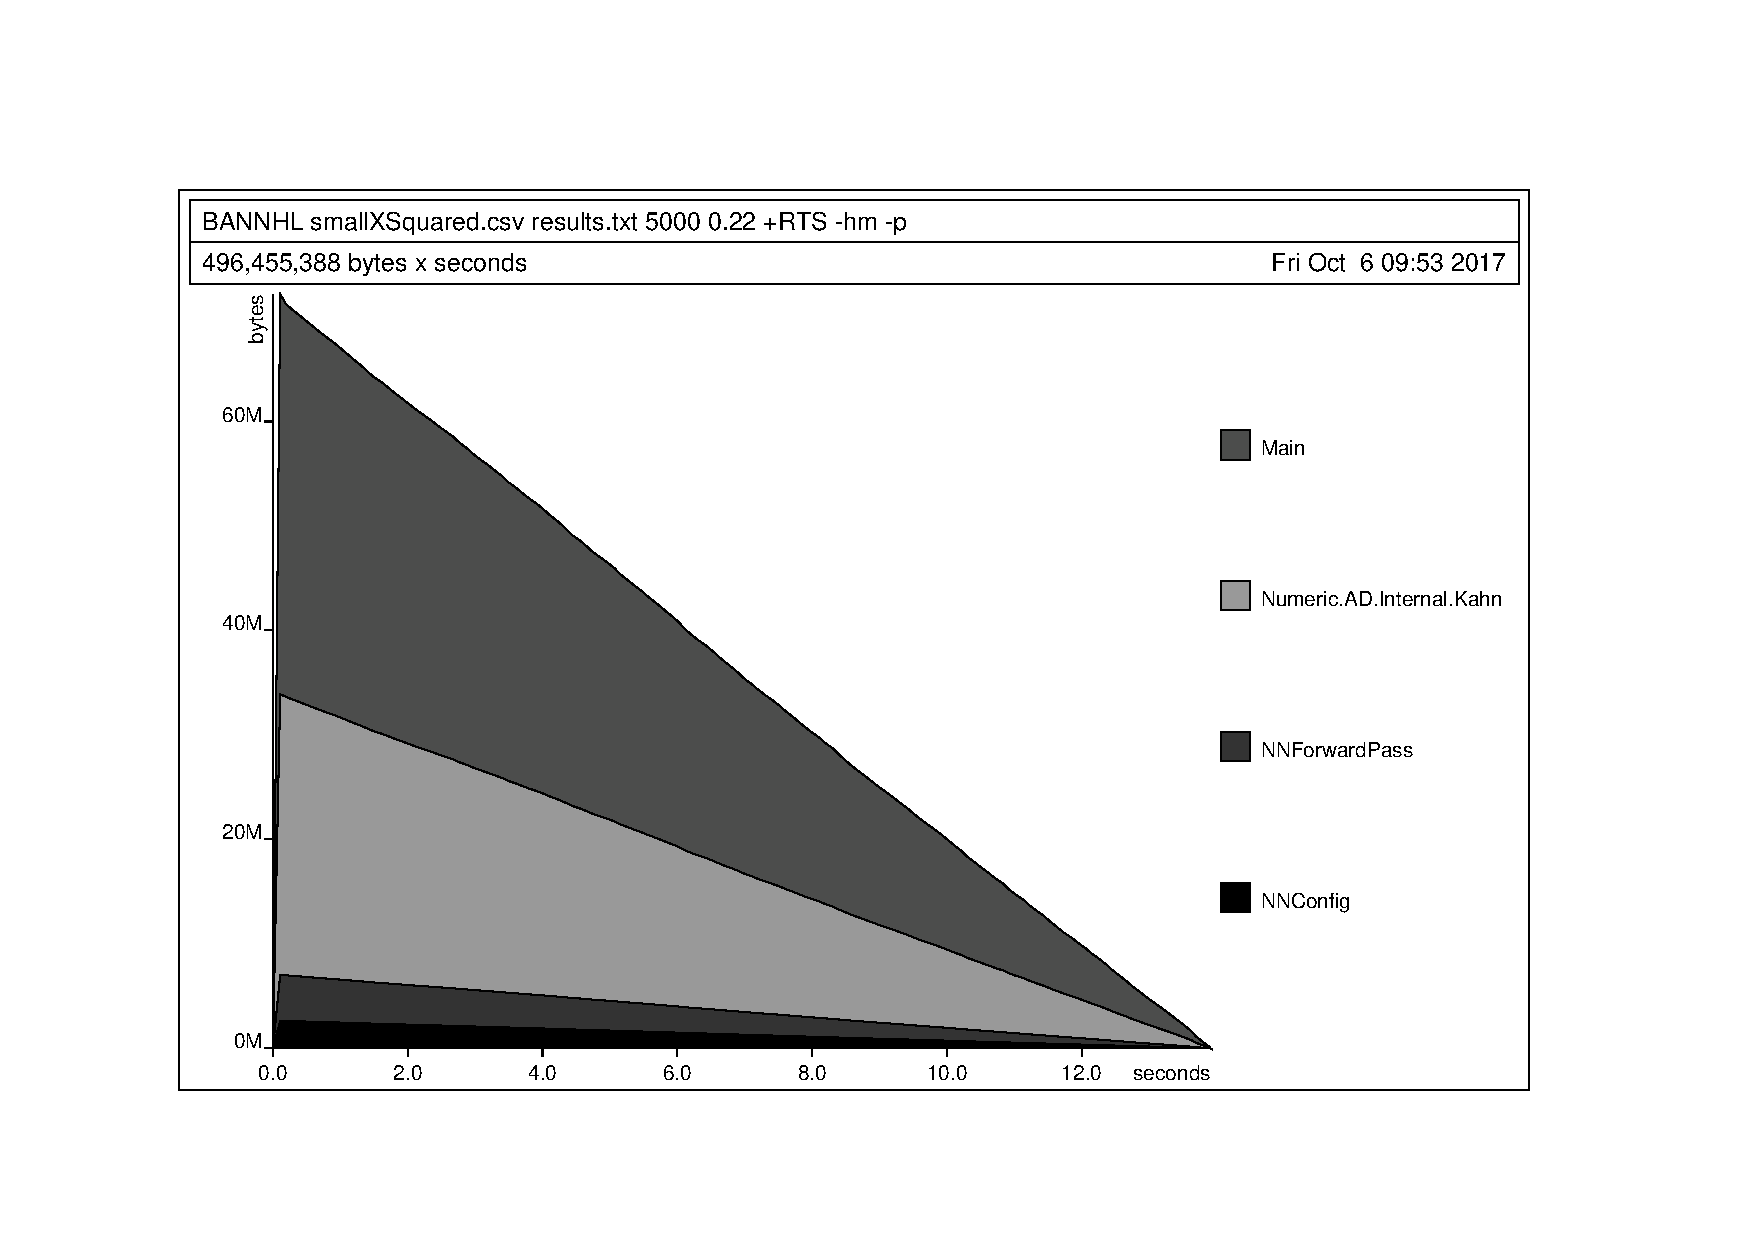
\includepdf[pages={1}]{data/heap-profile-BANNHL-by-module.pdf}
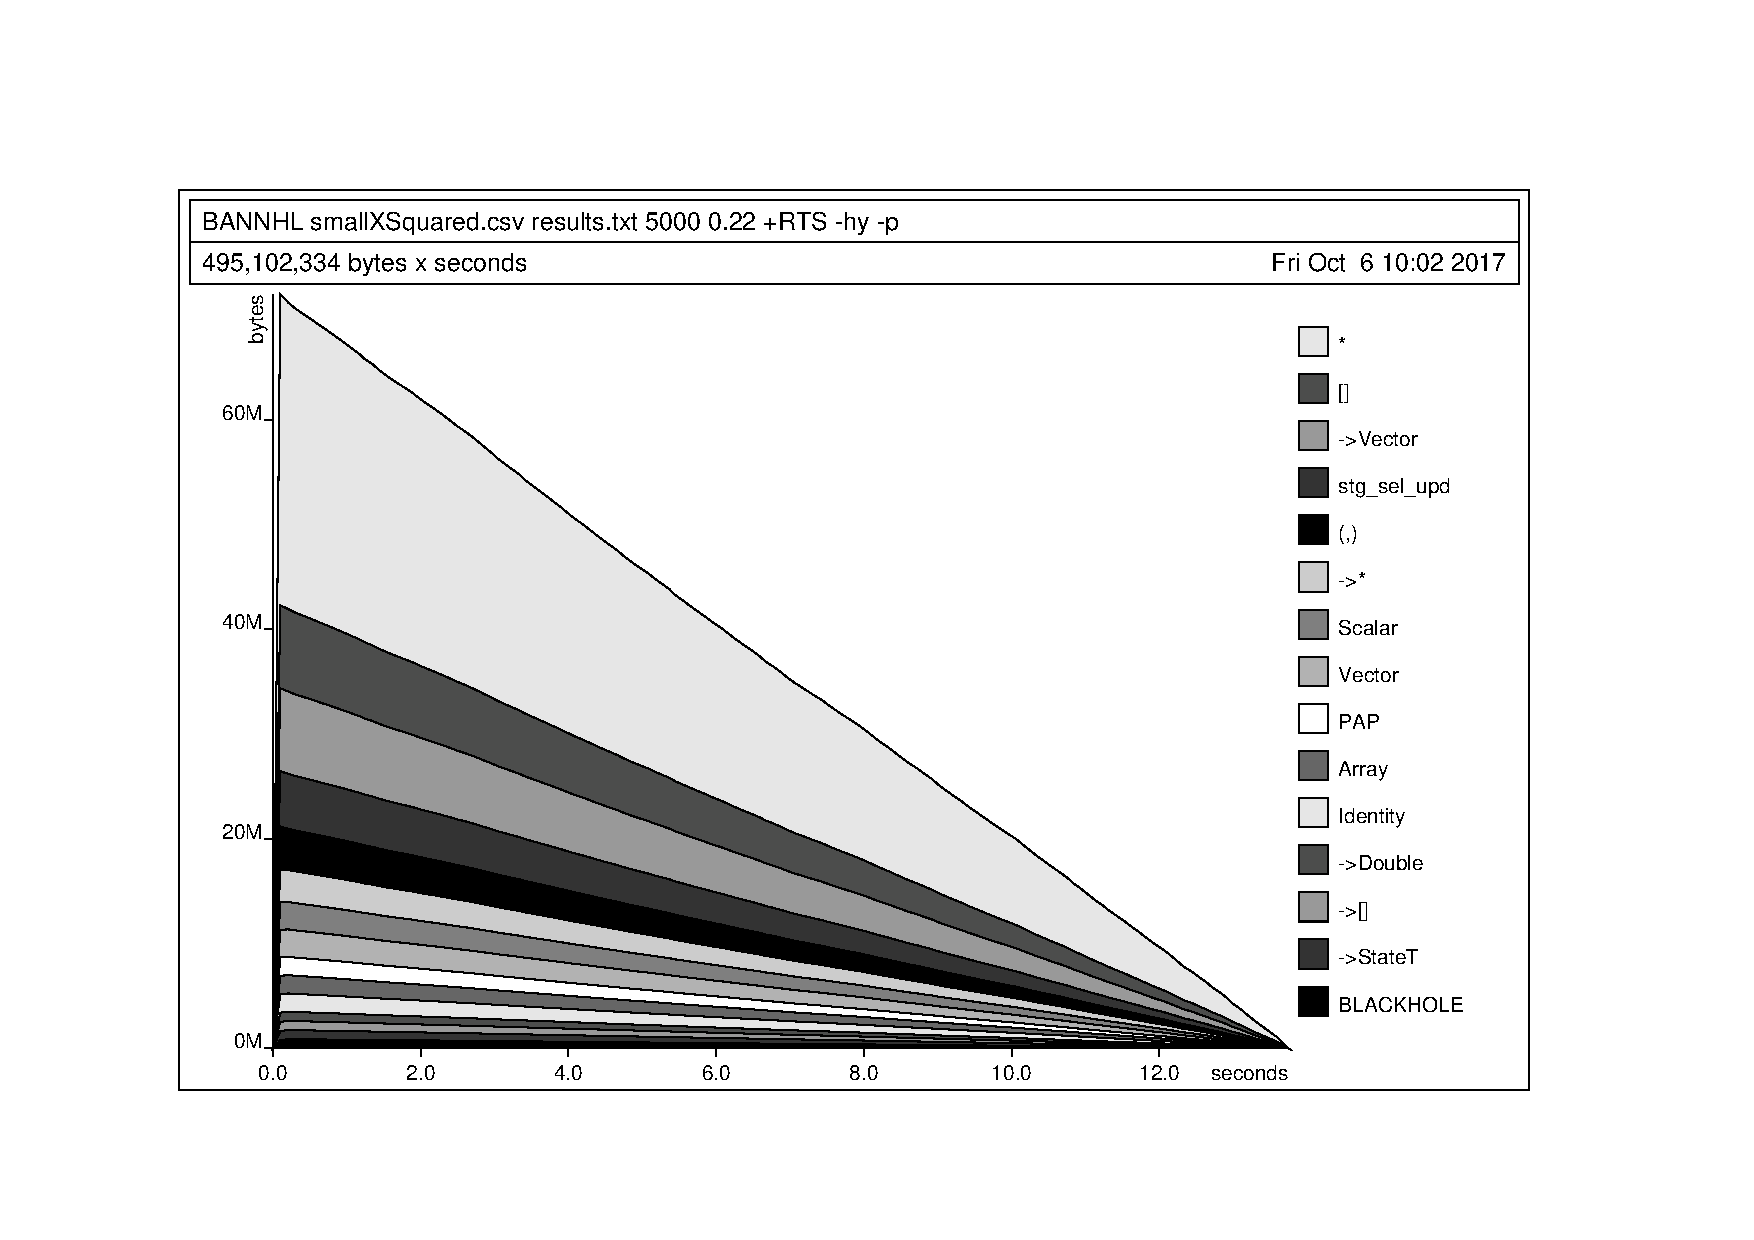
\includepdf[pages={1}]{data/heap-profile-BANNHL-by-type.pdf}
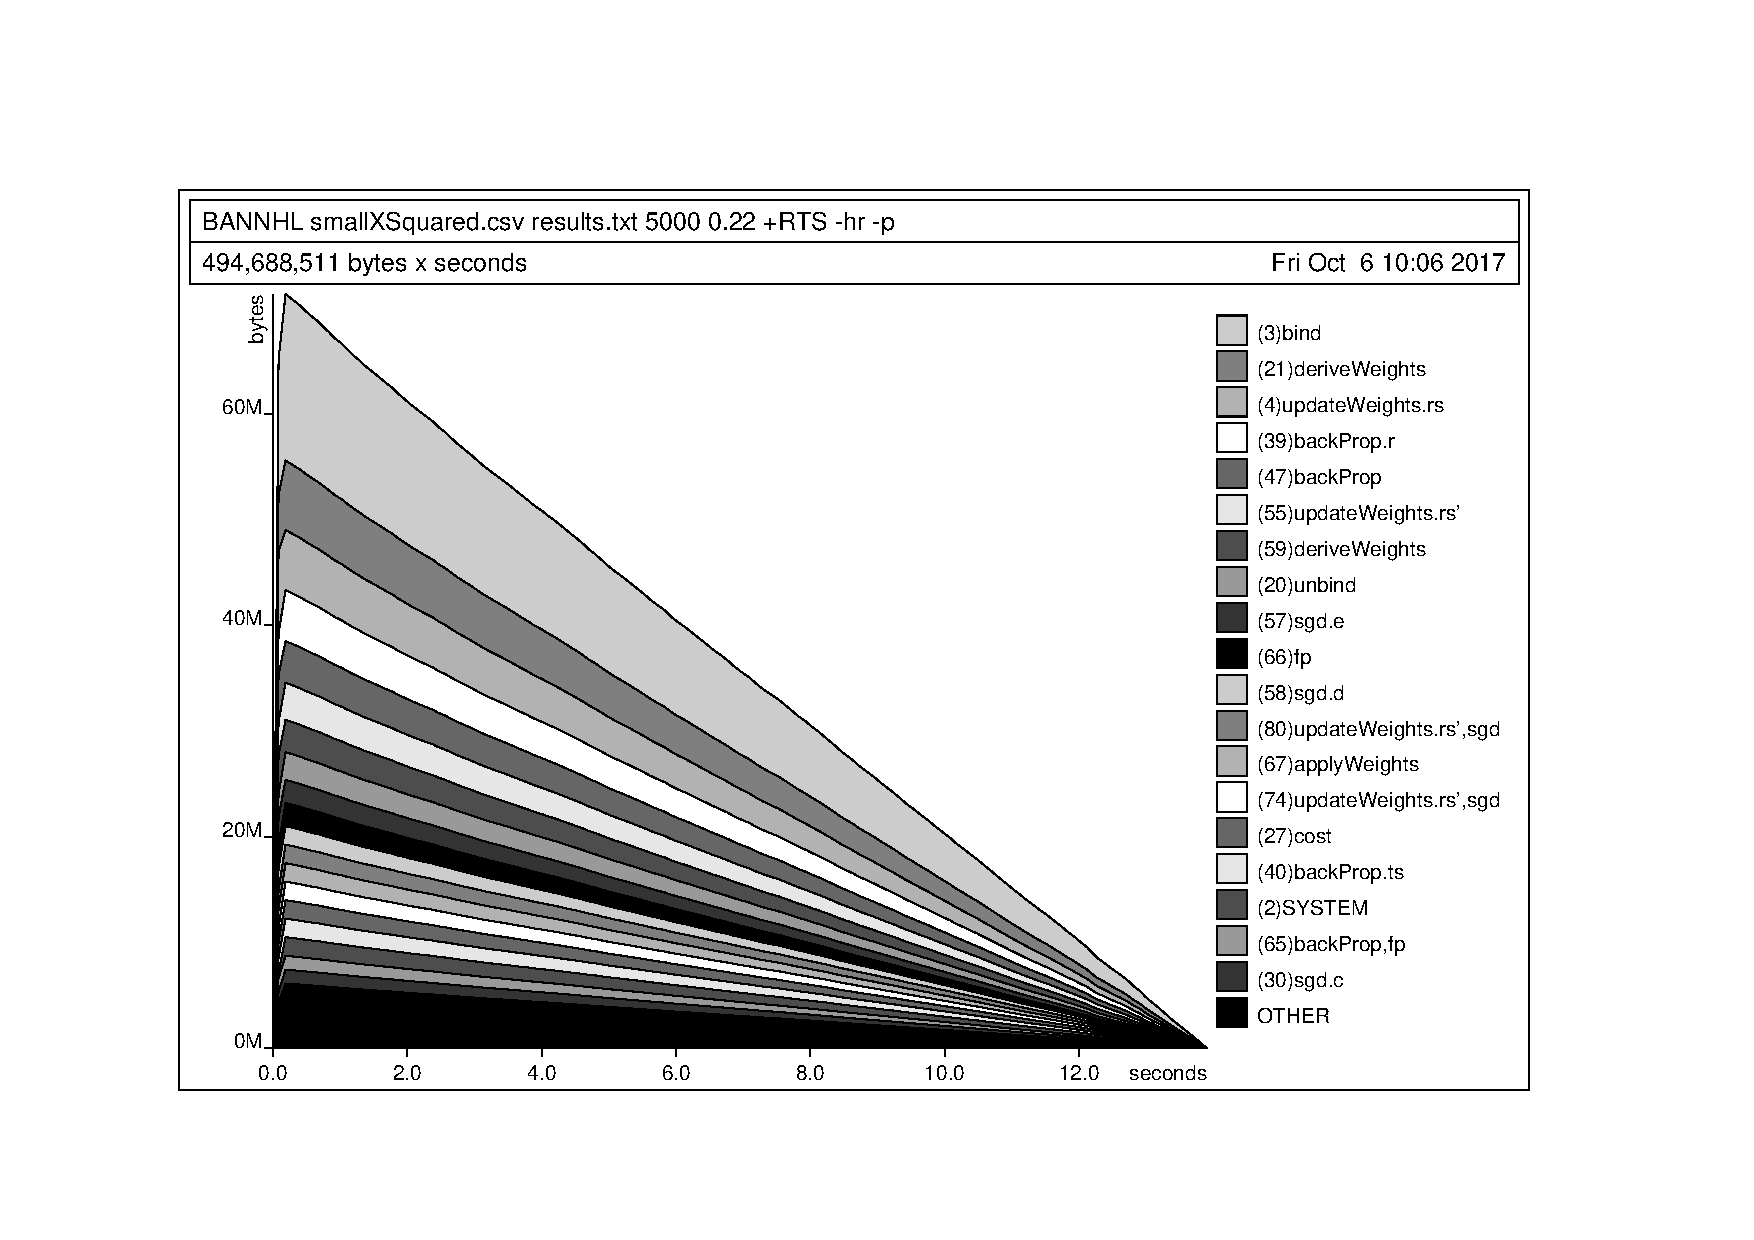
\includepdf[pages={1}]{data/heap-profile-BANNHL-by-retainer.pdf}
\subsection{Performance for BANNHL}
See BANNHL.prof included along with this report for the performance
breakdown of BANNHL.

\end{document}
